\documentclass[a4paper]{article}

\usepackage[left=1.5cm, right=1.5cm, top=1.5cm, bottom=1.5cm]{geometry} 
\usepackage[utf8]{inputenc} 
\usepackage{german} 
\usepackage{amsmath} 
\usepackage{amssymb} 
\usepackage{listings} 
\usepackage{hyperref} 
\usepackage{graphicx} 
\usepackage{eurosym} 
\usepackage{ulem} \DeclareUnicodeCharacter{20AC}{\euro}

% \usepackage{helvet}
\renewcommand{\familydefault}{\sfdefault}

\begin{document}

\begin{center}
    \begin{minipage}{.2\textwidth}
        \flushleft
        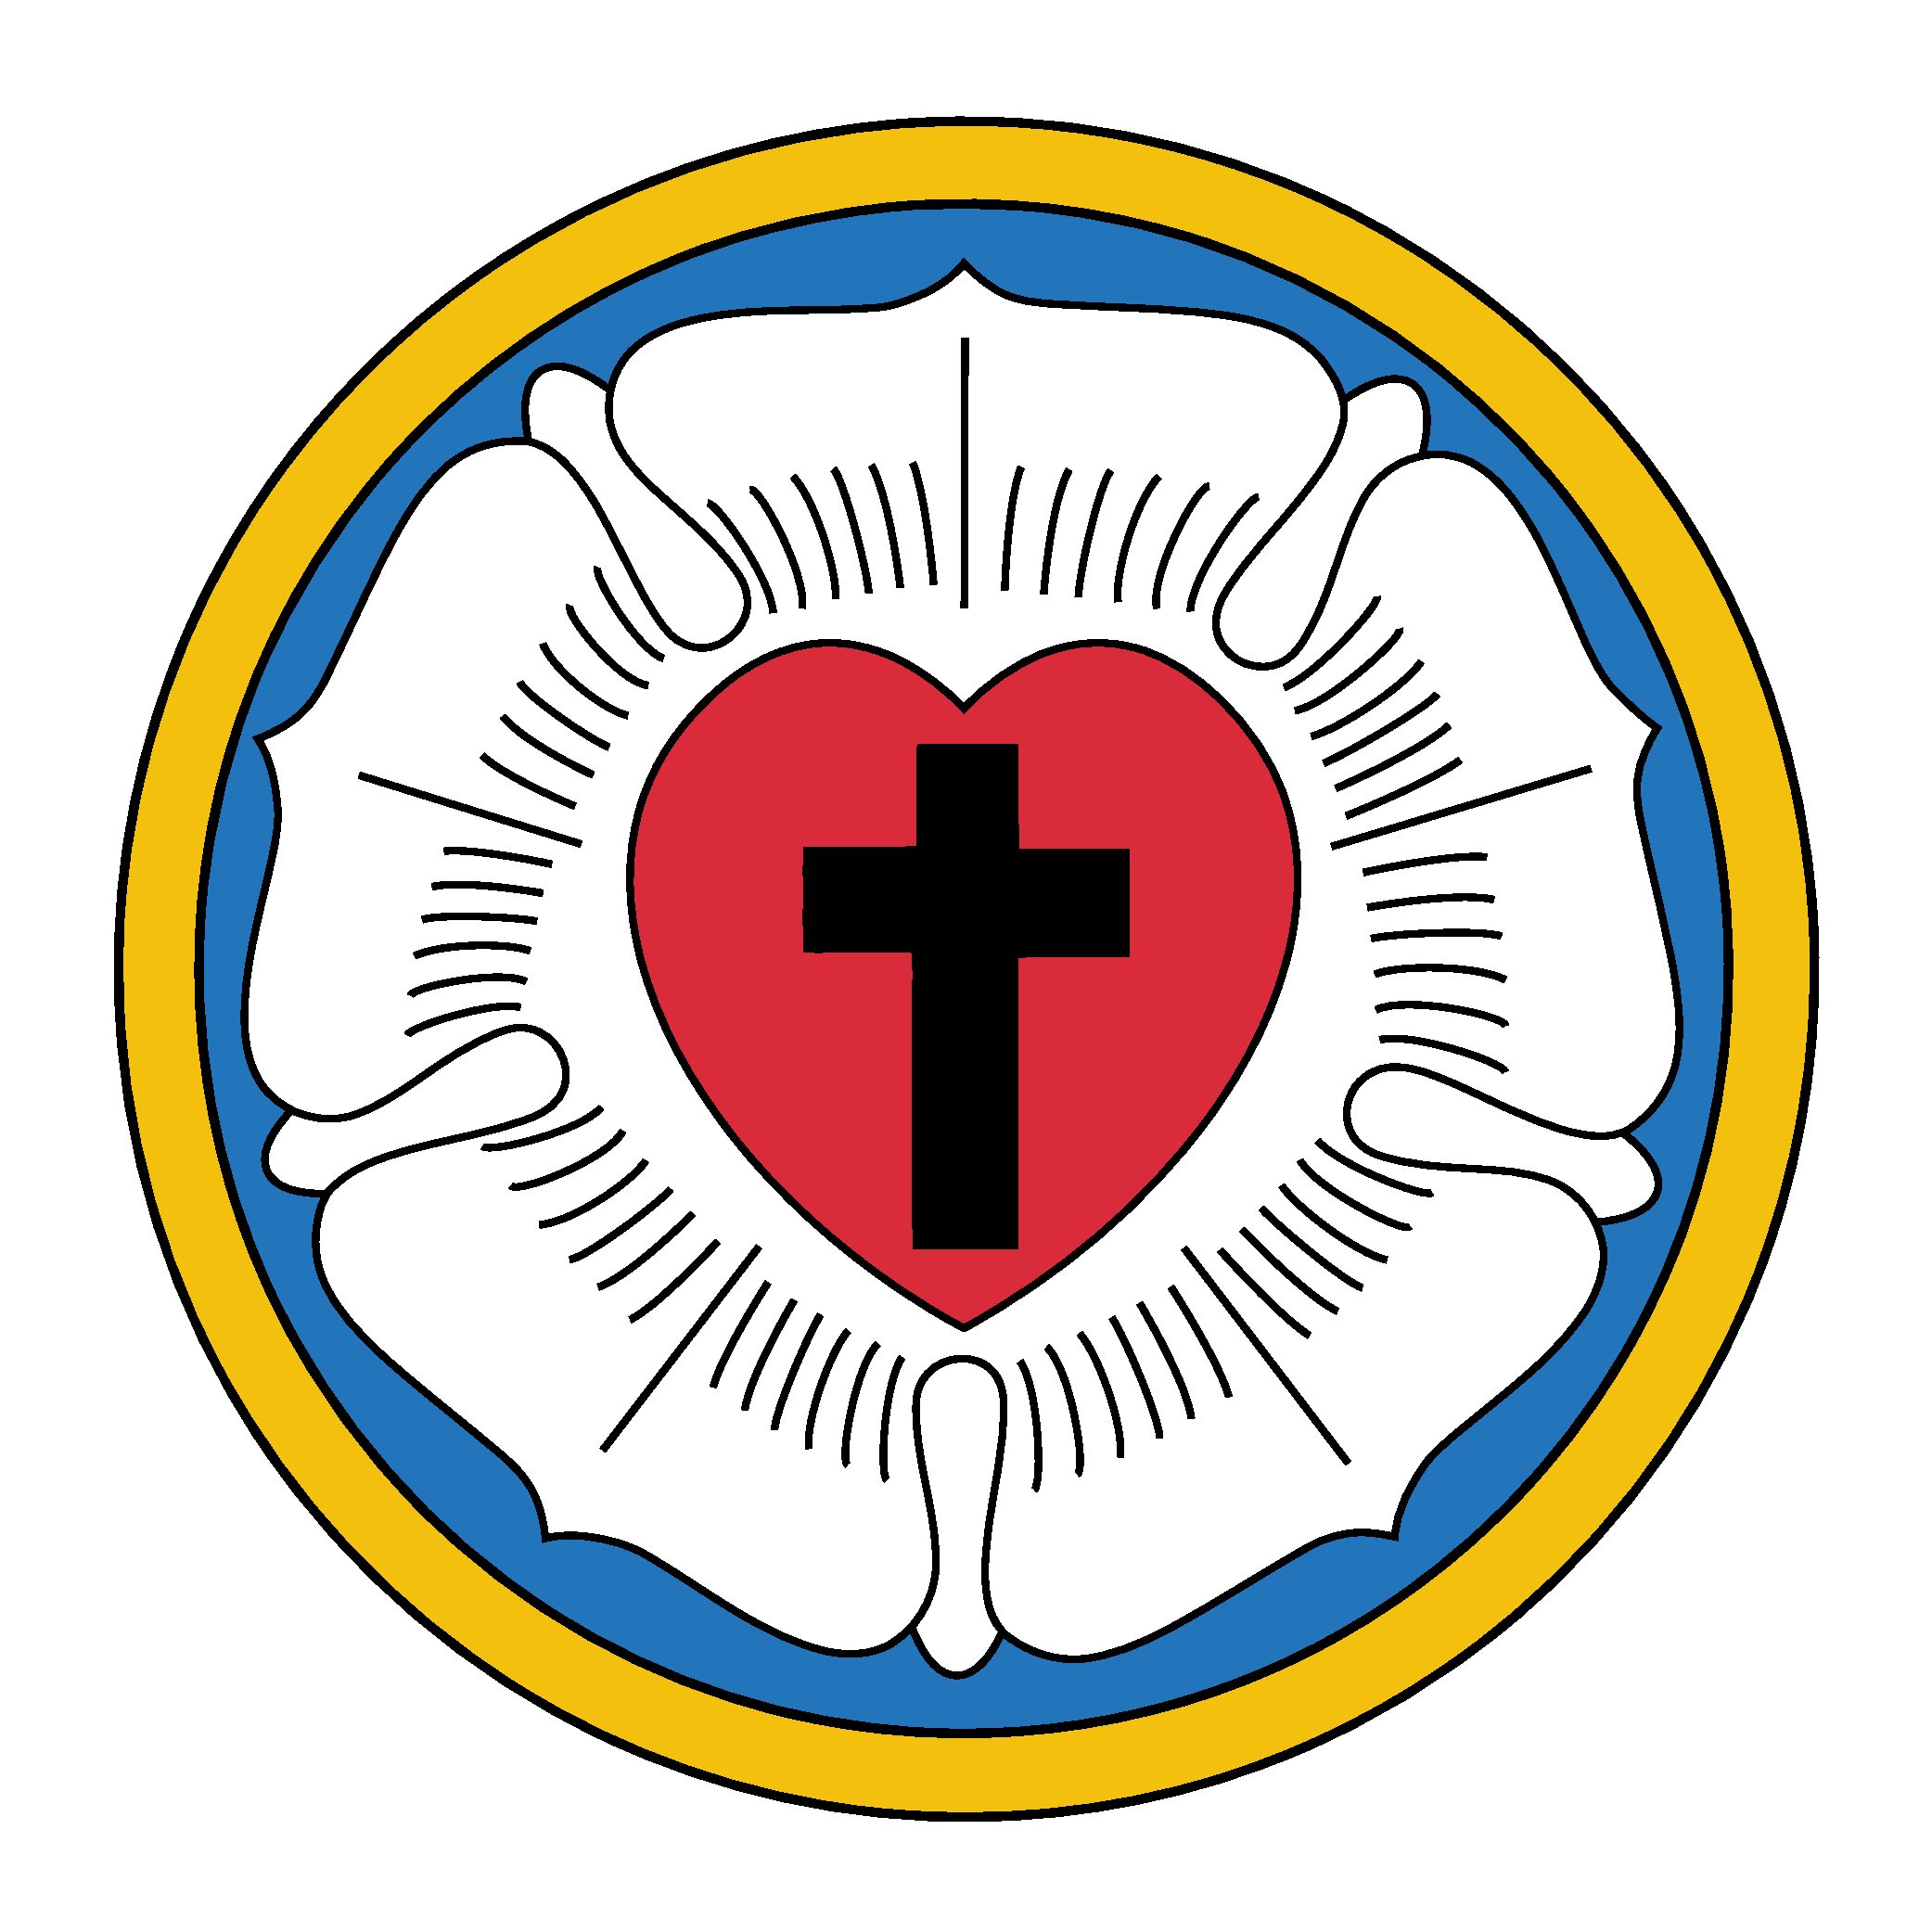
\includegraphics[width=1\linewidth]{Lutherrose.pdf}
    \end{minipage}%
    \begin{minipage}{.6\textwidth}
        \begin{center}
            \footnotesize Verband Christlicher Pfadfinderinnen und Pfadfinder\\
            \large Stamm Martin Luther Lumdatal\\
            ~\\
            \Large \textbf{Änderungsantrag zur Stammesordnung}\\
            \normalsize Anpassung der Stammesordnung an die Stufenordnung des VCP\\
            ~\\[1cm]
        \end{center}
    \end{minipage}%
    \begin{minipage}{.2\textwidth}
        \flushright
        
\includegraphics[width=.85\linewidth]{Zeichen.pdf}
    \end{minipage}%
\end{center}
~\\[0.5cm] 

\emph{Die Mitgliederversammlung möge beschließen die Stammesordnung wie folgt zu ändern:}

\section{Streichen von 3.2 Die Jungpfadfinderstufe}
    \begin{itemize}
        \item Die Jungpfadfinderstufe nimmt Kinder im Alter von 10 bis 13 Jahren auf. Mitglieder dieser Stufe werden als Jungpfadfinder bezeichnet.
        \item Die Arbeit erfolgt in kleinen Gruppen von 4 bis 10 Personen, die Sippen genannt werden. Alle Jungpfadfinder- und Pfadfindersippen des Stammes werden als Trupp bezeichnet.
        \item Jede Sippe besitzt einen Sippenführer, der für die Planung und Durchführung der Sippenstunden sowie sämtlicher anderer Aktionen der Sippe zuständig ist.
    \end{itemize}

\section{Streichen von 3.3 Die Pfadfinderstufe}
    \begin{itemize}
        \item Die Pfadfinderstufe nimmt Jugendliche im Alter von 13 bis 16 Jahren auf. Mitglieder dieser
Stufe werden als Pfadfinder bezeichnet.
        \item Die Strukturen der Jungpfadfinderstufe bleiben erhalten.
    \end{itemize}


\section{Einführen von 3.2 Die Pfadfinderstufe} % (fold)
\label{sec:anpassung_der_ordnung_auf_die_neue_beauftragung}
    \label{sub:die_pfadfinderstufe}
    \begin{itemize}
        \item Die Pfadfinderstufe ist für Kinder und Jugendliche im Alter von 10 bis 16 Jahren. 
        \item Die Arbeit erfolgt in kleinen Gruppen von 4 bis 10 Personen, die Sippen genannt werden. Alle Jungpfadfinder- und Pfadfindersippen des Stammes werden als Trupp bezeichnet.
        \item Jede Sippe besitzt einen Sippenführer, der für die Planung und Durchführung der Sippenstunden sowie sämtlicher anderer Aktionen der Sippe zuständig ist. 
        \item Die Pfadfinderstufe ist in zwei Phasen untergliedert:
        \subsubsection*{3.2.1 Jungpfadfinderphase} % (fold)
        \label{ssub:jungpfadfinderphase}
            \begin{itemize}
                \item Die Jungpfadfinderphase nimmt Kinder im Alter von 10 bis 13 auf. Sie tragen das hellgrün-blaue Halstuch 
                \item Schwerpunkt der Arbeit liegt auf dem zusammenwachsen der Gruppe und dem spielerischen Lernen. Sie nehmen an Veranstaltungen der Region und an entsprechenden Veranstaltungen des Landes teil.
            \end{itemize}
        % subsubsection jungpfadfinderphase (end)
        \subsubsection*{3.2.2 Pfadfinderphase} % (fold)
        \label{ssub:pfadfinderphase}
        \begin{itemize}
            \item Die Pfadfinderphase nimmt Jugendliche im Alter von 13 bis 16 auf. Mitglieder dieser Stufe tragen das dunkelgrün-blaue Halstuch.
            \item In der Pfadfinderphase übernehmen die Jugendlichen eigene Verantwortung. Schwerpunkt ist weiterhin die kleine Gruppe, aber auch die persönliche Entwicklung des einzelnen.
        \end{itemize}
        % subsubsection pfadfinderphase (end)
    \end{itemize}

\clearpage
\section{Weitere Änderungen} % (fold)
\label{sec:weitere_anderungen}
\begin{table}[h]
\def\arraystretch{2}
\center
\begin{tabular}{ l|p{.45\textwidth}|p{.45\textwidth}}
    \# & \textbf{Stammesordnung 2014}                                            & \textbf{geänderte Version}                                                                                         \\ \hline
    1  & Die Kinderstufe nimmt Kinder im Alter von 7 bis 10 Jahren auf.          & Die Kinderstufe nimmt Kinder im Alter von 7 bis 10 Jahren auf. Sie tragen das rot-blaue Halstuch.                  \\\hline
    2  & Die Ranger/Rover Stufe nimmt Jugendliche im Alter von 16-21 Jahren auf. & Die Ranger/Rover Stufe nimmt Jugendliche im Alter von 16-21 Jahren auf. Sie tragen das bordeauxrot-blaue Halstuch. \\\hline
    3  & (nicht vorhanden)                                                       & Die Mitglieder der Erwachsenenarbeit tragen das violett-blaue Halstuch.                                           
    \end{tabular}
\end{table}
% section weitere_anderungen (end)

~\\[0.5cm]
{\emph{Begründung zum Antrag: }
Unsere Stammesordnung entspricht nicht der Stufenkonzeption des VCP, obwohl wir uns zu Anfang des Absatz zu dieser bekennen: ''Der Stamm Martin Luther Lumdatal erkennt die Stufenkonzeption des VCP ohne Einschränkungen an...''
\end{document}






